\documentclass[14pt]{beamer}
\usepackage{./Estilos/BeamerUVM}
\usepackage{./Estilos/ColoresLatex}
\usetheme{Madrid}
\usecolortheme{default}
%\useoutertheme{default}
\setbeamercovered{invisible}
% or whatever (possibly just delete it)
\setbeamertemplate{section in toc}[sections numbered]
\setbeamertemplate{subsection in toc}[subsections numbered]
\setbeamertemplate{subsection in toc}{\leavevmode\leftskip=3.2em\rlap{\hskip-2em\inserttocsectionnumber.\inserttocsubsectionnumber}\inserttocsubsection\par}
% \setbeamercolor{section in toc}{fg=blue}
% \setbeamercolor{subsection in toc}{fg=blue}
% \setbeamercolor{frametitle}{fg=blue}
\setbeamertemplate{caption}[numbered]

\setbeamertemplate{footline}
\beamertemplatenavigationsymbolsempty
\setbeamertemplate{headline}{}


\makeatletter
% \setbeamercolor{section in foot}{bg=gray!30, fg=black!90!orange}
% \setbeamercolor{subsection in foot}{bg=blue!30}
% \setbeamercolor{date in foot}{bg=black}
\setbeamertemplate{footline}
{
  \leavevmode%
  \hbox{%
  \begin{beamercolorbox}[wd=.333333\paperwidth,ht=2.25ex,dp=1ex,center]{section in foot}%
    \usebeamerfont{section in foot} {\insertsection}
  \end{beamercolorbox}%
  \begin{beamercolorbox}[wd=.333333\paperwidth,ht=2.25ex,dp=1ex,center]{subsection in foot}%
    \usebeamerfont{subsection in foot}  \insertsubsection
  \end{beamercolorbox}%
  \begin{beamercolorbox}[wd=.333333\paperwidth,ht=2.25ex,dp=1ex,right]{date in head/foot}%
    \usebeamerfont{date in head/foot} \insertshortdate{} \hspace*{2em}
    \insertframenumber{} / \inserttotalframenumber \hspace*{2ex} 
  \end{beamercolorbox}}%
  \vskip0pt%
}
\makeatother

\makeatletter
\patchcmd{\beamer@sectionintoc}{\vskip1.5em}{\vskip0.8em}{}{}
\makeatother

% \usefonttheme{serif}
\usepackage[clock]{ifsym}

\sisetup{per-mode=symbol}
\DeclareSIUnit{\dB}{dB}
\resetcounteronoverlays{saveenumi}

\title{\Large{Ondas sonoras} \\ \normalsize{Física IV (área II)}}
\date{}

% Macro para agregar el logo de UVM en cada slide de la presentación

\addtobeamertemplate{frametitle}{}{%
\begin{tikzpicture}[remember picture,overlay]
\coordinate (logo) at ([xshift=-1.5cm,yshift=-0.8cm]current page.north east);
% \fill[devryblue] (logo) circle (.9cm);
% \clip (logo) circle (.75cm);
\node at (logo) {
\includegraphics[width=2.1cm]{Imagenes/logo_UVM.png}};
\end{tikzpicture}}


\begin{document}
\maketitle

\section*{Contenido}
\frame[allowframebreaks]{\frametitle{Contenido} \tableofcontents[currentsection, hideallsubsections]}

\section{El sonido}
\frame{\tableofcontents[currentsection, hideothersubsections]}
\subsection{Definición}

\begin{frame}
\frametitle{¿Qué es el sonido?}
El \textocolor{carmine}{sonido} es el fenómeno físico que estimula al oído.
\end{frame}
\begin{frame}
\frametitle{Frecuencias audibles}    
En los seres humanos, el sonido se percibe cuando un cuerpo vibra a una \textocolor{cobalt}{frecuencia} comprendida entre 15 y \SI{20000}{\hertz} y llega al oído interno: \pause gama denominada de frecuencias del \textocolor{darkcyan}{espectro audible}.
\end{frame}
\begin{frame}
\frametitle{Frecuencias audibles}    
Cuando la frecuencia de una onda sonora es \textocolor{darkorchid}inferior al límite audible, \pause se dice que es \textocolor{darkorchid}{infrasónica} \pause y si es \textocolor{darkgreen}{mayor es ultrasónica}.
\end{frame}
\begin{frame}
\frametitle{El sonido como onda longitudinal}
Las ondas sonoras son \textocolor{bronze}{ondas mecánicas longitudinales}, toda vez que las partículas del medio material vibran paralelamente a la dirección de propagación de la onda.
\end{frame}
\begin{frame}
\frametitle{El sonido como onda longitudinal}
\begin{figure}
    \centering
    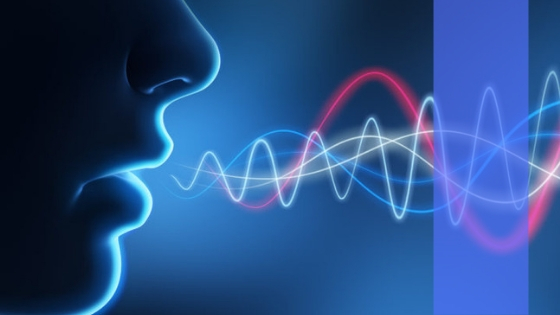
\includegraphics[scale=0.6]{Imagenes/Sonido_01.jpg}
\end{figure}
\end{frame}
\begin{frame}
\frametitle{Propagación del sonido}
Como el sonido se transmite en todas las direcciones en forma de ondas, por medio de cualquier material elástico, se trata de ondas tridimensionales o espaciales.
\end{frame}
\begin{frame}
\frametitle{Medio necesario para transmitirse}
Un sonido, por intenso que sea, \textocolor{red}{no se propaga en el vacío} porque no existe en éste un material por el cual se transmita la vibración.
\end{frame}

\section{Velocidad del sonido}
\frame{\tableofcontents[currentsection, hideothersubsections]}
\subsection{Medio y temperatura}

\begin{frame}
\frametitle{La velocidad del sonido}
La \textocolor{blue-violet}{rapidez} con la que se propaga un sonido depende del \textocolor{burntorange}{medio elástico} y de su \textocolor{byzantium}{temperatura}.
\end{frame}
\begin{frame}
\frametitle{La velocidad del sonido}
\begin{table}
\renewcommand{\arraystretch}{0.8}
\centering
\begin{tabular}{c | c | c }
Medio elástico & Rapidez [\unit{\meter\per\second}] & Temperatura [\unit{\kelvin}] \\ \hline
Aire & \num{331.4} & \num{273} \\ \hline
Aire & \num{340} & \num{288} \\ \hline
Agua & \num{1435} & \num{281} \\ \hline
Oxígeno & \num{317} & \num{273} \\ \hline
Hierro & \num{5130} & \num{293} \\ \hline
Aluminio & \num{5100} & \num{293} \\ \hline
Vidrio & \num{4500} & \num{293} \\ \hline
\end{tabular}
\end{table}
\end{frame}
\begin{frame}
\frametitle{Conversión de temperatura}
Recordemos que para obtener la temperatura en grados centígrados, hacemos la operación:
\pause
\begin{align*}
\unit{\degreeCelsius} = K - 273
\end{align*}
\end{frame}

\section{Fenómenos acústicos}
\frame{\tableofcontents[currentsection, hideothersubsections]}
\subsection{La acústica}

\begin{frame}
\frametitle{¿Qué es la acústica?}
La \textocolor{darkslateblue}{acústica} es la parte de la Física que se encarga del estudio de los sonidos.
\end{frame}
\begin{frame}
\frametitle{Los fenómenos acústicos}
Los fenómenos acústicos, consecuencia de algunos efectos auditivos provocados por el sonido, son:
\pause
\setbeamercolor{item projected}{bg=guppiegreen,fg=black}
\setbeamertemplate{enumerate items}{%
\usebeamercolor[bg]{item projected}%
\raisebox{1.5pt}{\colorbox{bg}{\color{fg}\footnotesize\insertenumlabel}}%
}
\begin{enumerate}[<+->]
\item Reflexión.
\item Eco.
\item Resonancia.
\item Reverberación.
\end{enumerate}
\end{frame}

\subsection{Reflexión}

\begin{frame}
\frametitle{La reflexión}
Este fenómeno se produce cuando las ondas sonoras se \textocolor{indigo(web)}{reflejan} al chocar contra una pared dura.
\end{frame}
\begin{frame}
\frametitle{La reflexión}
Si el \textocolor{internationalorange}{vector de propagación sonoro} incide \textocolor{islamicgreen}{perpendicularmente} a una superficie, \pause se refleja en sentido contrario.
\end{frame}
\begin{frame}
\frametitle{Representando la reflexión}
\begin{figure}
    \centering
    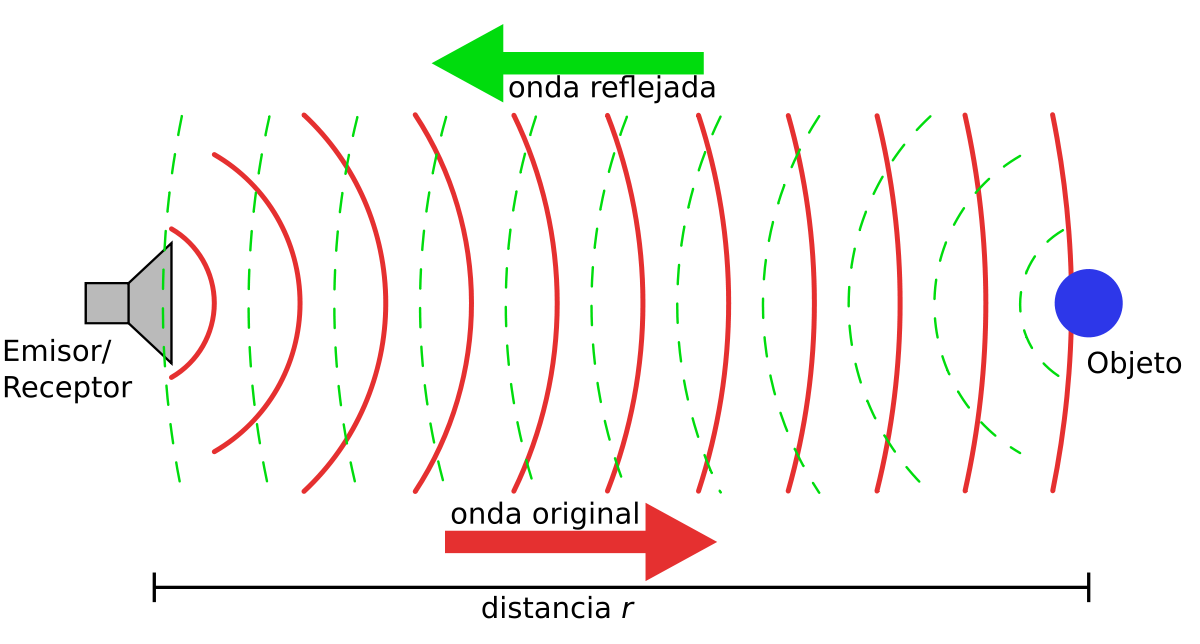
\includegraphics[scale=0.2]{Imagenes/Acustica_01.png}
\end{figure}
\end{frame}
\begin{frame}
\frametitle{La reflexión}
Pero si incide en forma oblicua, los ángulos de incidencia y de reflexión son iguales.
\end{frame}
\begin{frame}
\frametitle{Representando la reflexión}
\begin{figure}
    \centering
    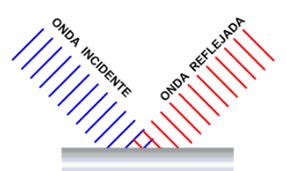
\includegraphics[scale=0.6]{Imagenes/Acustica_02.jpg}
\end{figure}
\end{frame}

\subsection{Eco}

\begin{frame}
\frametitle{Definición del eco}
El\textocolor{darkgreen}{eco} Se origina cuando una onda se \textocolor{coquelicot}{refleja} y regresa a su emisor.
\end{frame}
\begin{frame}
\frametitle{Eel eco}
\begin{figure}
    \centering
    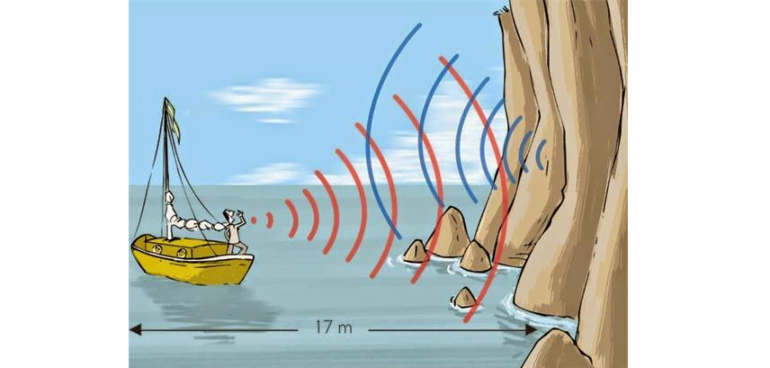
\includegraphics[width = \linewidth]{Imagenes/Eco_01.png}
\end{figure}
\end{frame}
\begin{frame}
\frametitle{Usos del eco}
Una aplicación del eco se tiene al medir la profundidad del mar, usando un aparato llamado sonar.
\end{frame}
\begin{frame}
\frametitle{Ecolocalización}
Algunos animales ocupan la \textocolor{crimsonglory}{ecolocalización} para detectar a sus presas.
\end{frame}
\begin{frame}
\frametitle{Ecolocalización}
\begin{figure}
    \centering
    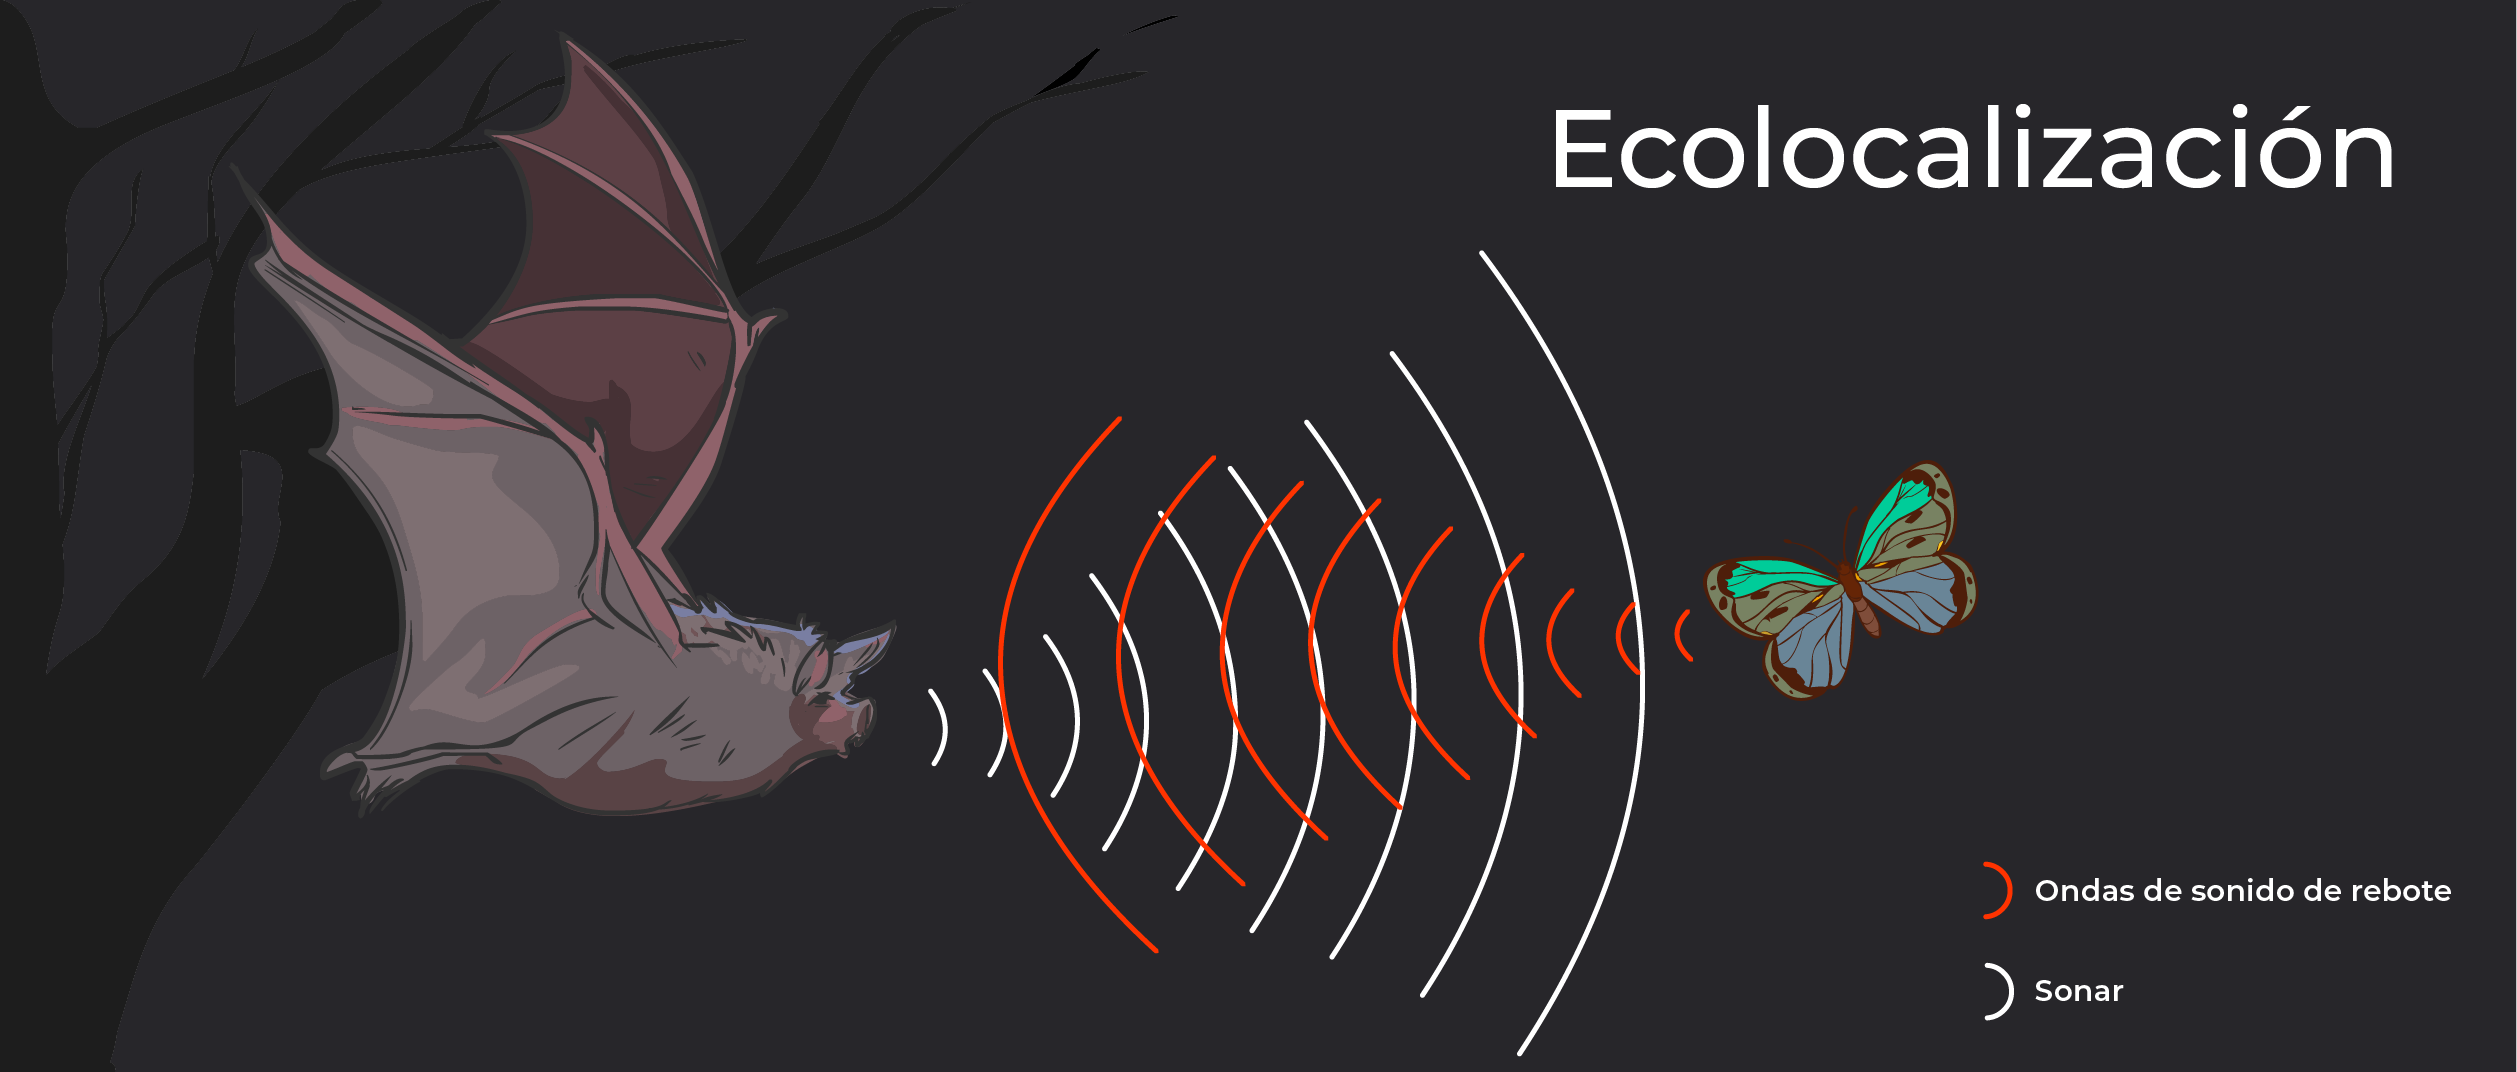
\includegraphics[width = \linewidth]{Imagenes/Eco_02b.png}
\end{figure}
\end{frame}
\begin{frame}
\frametitle{Ecolocalización}
\begin{figure}
    \centering
    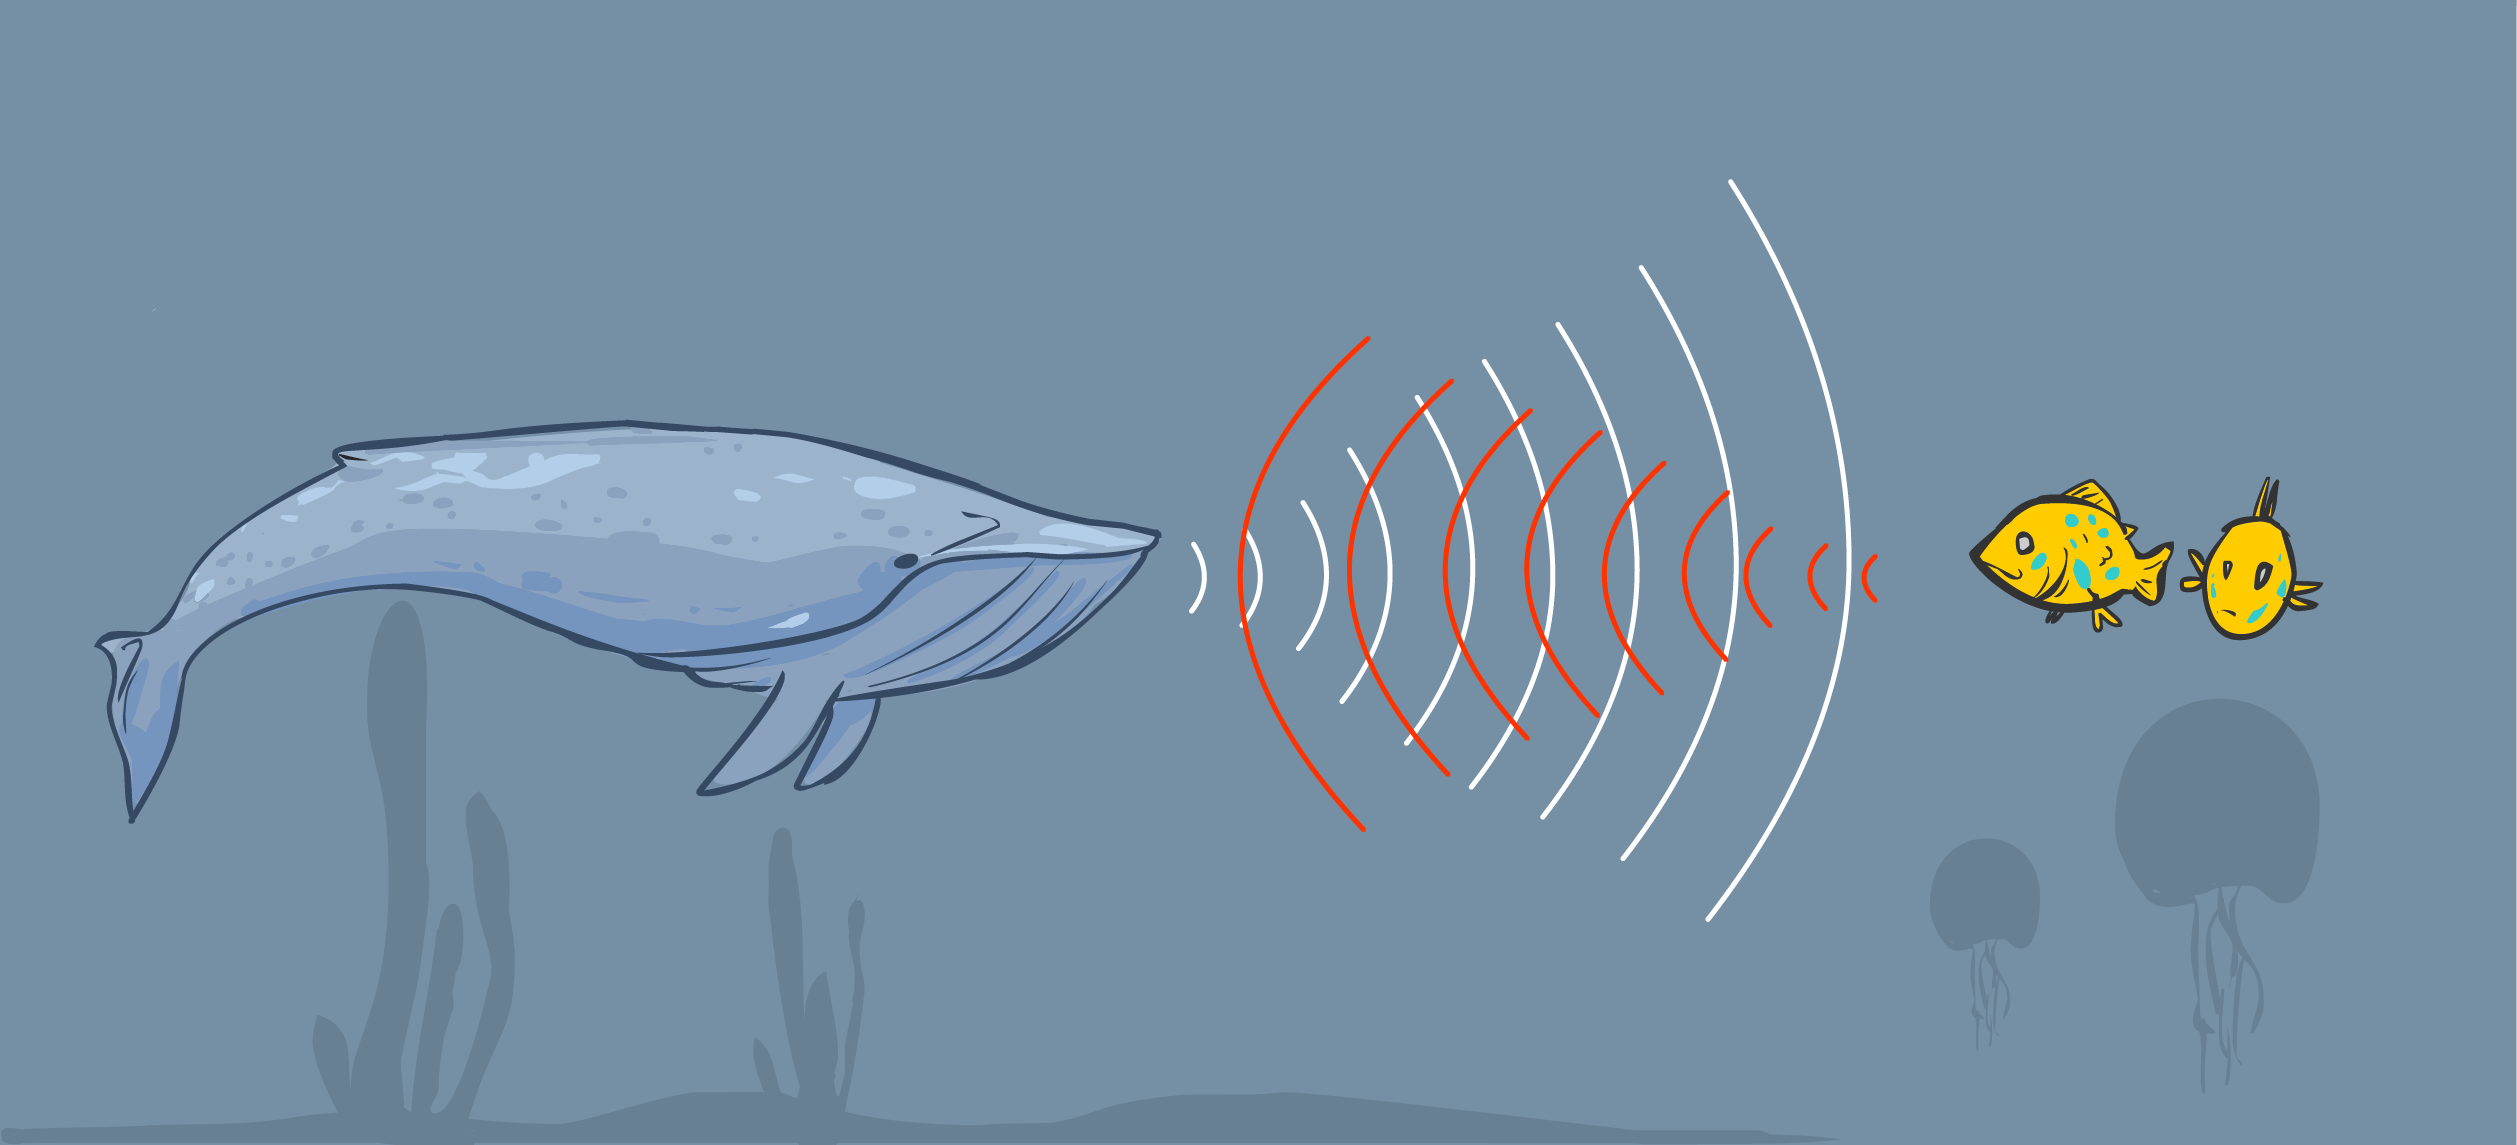
\includegraphics[width = \linewidth]{Imagenes/Eco_02c.png}
\end{figure}
\end{frame}

\subsection{Resonancia}

\begin{frame}
\frametitle{Definición de Resonancia}
La \textocolor{darklavender}{resonancia} se presenta cuando la vibración de un cuerpo hace vibrar a otro con la \textocolor{ferrarired}{misma frecuencia}.
\end{frame}
\begin{frame}
\frametitle{Resonancia acústica}
\begin{figure}
    \centering
    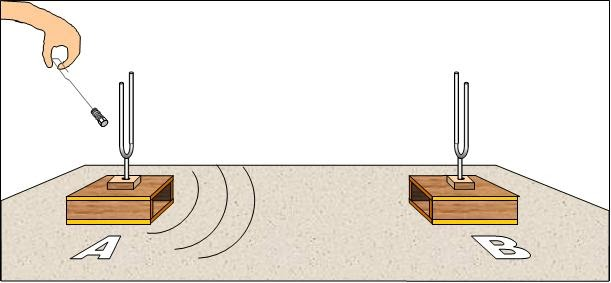
\includegraphics[width=\linewidth]{Imagenes/Resonancia_01.jpg}
\end{figure}
\end{frame}
\begin{frame}
\frametitle{Ejemplos de Resonancia}
Este fenómeno se ocupa en las llamadas \textocolor{jasper}{cajas de resonancia} que tienen algunos instrumentos musicales para aumentar la intensidad del sonido original.
\end{frame}
\begin{frame}
\frametitle{Resonancia acústica}
\begin{figure}
    \centering
    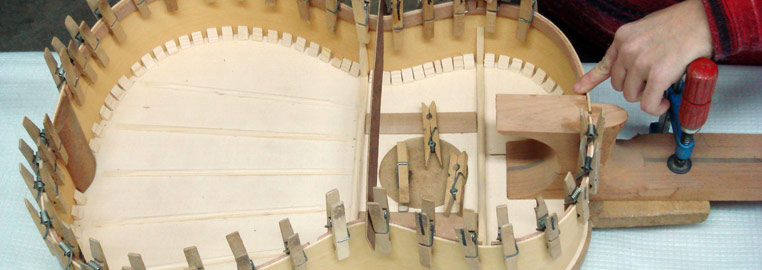
\includegraphics[width=\linewidth]{Imagenes/Resonancia_02.jpg}
\end{figure}
\end{frame}
\begin{frame}
\frametitle{Resonancia acústica}
\begin{figure}
    \centering
    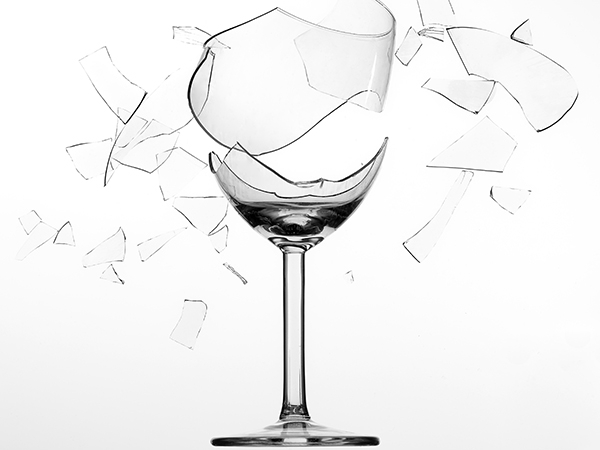
\includegraphics[scale=0.4]{Imagenes/Resonancia_03.jpg}
\end{figure}
\end{frame}

\subsection{Reverberación}

\begin{frame}
\frametitle{¿Qué es la reverberación?}
La \textocolor{regalia}{reverberación} se produce por la \textocolor{lava}{reflexión} \pause si después de escucharse un sonido original, éste persiste dentro de un local como consecuencia del eco.
\end{frame}
\begin{frame}
\frametitle{Ejemplo de la reverberación}
\begin{figure}
    \centering
    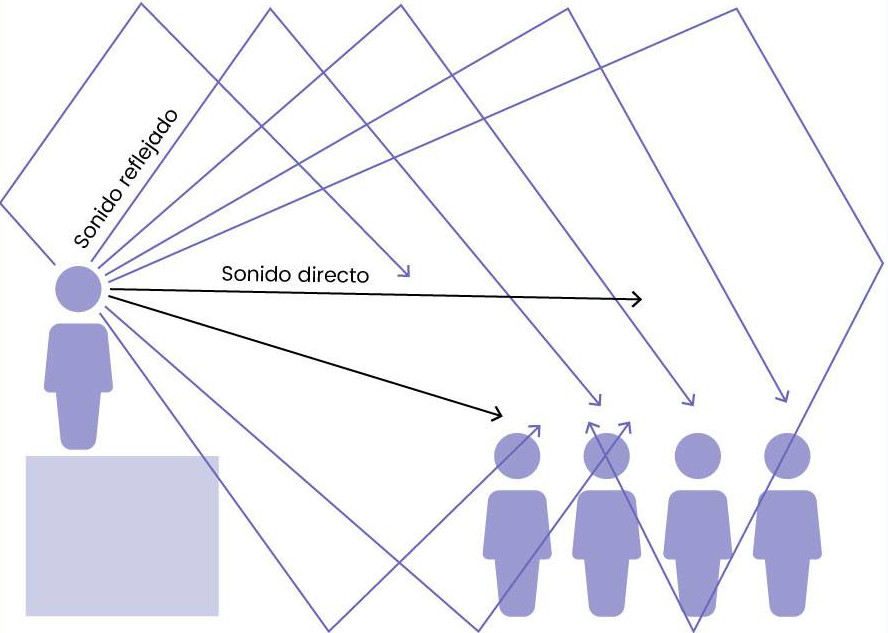
\includegraphics[scale=0.9]{Imagenes/Reverberacion_01.jpg}
\end{figure}
\end{frame}
\begin{frame}
\frametitle{Ejemplo de la reverberación}
En una sala amplia una reverberación excesiva ocasiona que no se escuchen claramente los sonidos producidos por instrumentos musicales, o la voz de las personas.
\end{frame}

\section{Cualidades del sonido}
\frame{\tableofcontents[currentsection, hideothersubsections]}
\subsection{Intensidad}

\begin{frame}
\frametitle{La intensidad}
La \textocolor{ruddy}{intensidad} determina si un sonido es fuerte o débil.
\end{frame}
\begin{frame}
\frametitle{La intensidad}
La intensidad de un sonido depende de:
\setbeamercolor{item projected}{bg=sunset,fg=black}
\setbeamertemplate{enumerate items}{%
\usebeamercolor[bg]{item projected}%
\raisebox{1.5pt}{\colorbox{bg}{\color{fg}\footnotesize\insertenumlabel}}%
}
\begin{enumerate}[<+->]
\item La \textocolor{sangria}{amplitud} de la onda, ya que a medida que esta aumenta, la intensidad también aumenta
\seti
\end{enumerate}
\end{frame}
\begin{frame}
\frametitle{La intensidad}
\setbeamercolor{item projected}{bg=sunset,fg=black}
\setbeamertemplate{enumerate items}{%
\usebeamercolor[bg]{item projected}%
\raisebox{1.5pt}{\colorbox{bg}{\color{fg}\footnotesize\insertenumlabel}}%
}
\begin{enumerate}[<+->]    
\conti
\item La \textocolor{tealgreen}{distancia} existente entre la fuente sonora y el oyente, pues a mayor distancia, menor intensidad.
\seti
\end{enumerate}
\end{frame}
\begin{frame}
\frametitle{La intensidad}
\setbeamercolor{item projected}{bg=sunset,fg=black}
\setbeamertemplate{enumerate items}{%
\usebeamercolor[bg]{item projected}%
\raisebox{1.5pt}{\colorbox{bg}{\color{fg}\footnotesize\insertenumlabel}}%
}
\begin{enumerate}[<+->]    
\conti
\item La \textocolor{applegreen}{intensidad es mayor} \pause si la \textocolor{violet}{superficie} que vibra también lo es.
\end{enumerate}
\end{frame}
\begin{frame}
\frametitle{Intesidad de sonido}
La intensidad de un sonido expresa la \textocolor{auburn}{cantidad de energía acústica} que en un segundo pasa a través de una superficie de un centímetro cuadrado, perpendicular a la dirección en la cual se propaga la onda.
\end{frame}
\begin{frame}
\frametitle{Intesidad de sonido}
Las unidades de intensidad sonora (Is) son:
\pause
\begin{align*}
Is = \dfrac{\unit{\joule\per\second}}{\SI{1}{\square\centi\meter}} = \dfrac{\unit{\watt}}{\unit{\square\centi\meter}}
\end{align*}
\end{frame}
\begin{frame}
\frametitle{Algunos valores de intensidad}
\begin{table}
    \renewcommand{\arraystretch}{0.8}
    \centering
    \begin{tabular}{c | c }
        $Is$ & Ejemplo \\ \hline
        \num{d-11} & Crujido de hojas \\ \hline
        \num{d-10} & Conversación suave a \SI{1}{\meter} \\ \hline
        \num{d-7} & Oficina suave, música suave \\ \hline
        \num{d-6} & Conversación normal \\ \hline
        \num{d-5} & Oficina ruidosa, tráfico pesado \\ \hline
    \end{tabular}
\end{table}
\end{frame}
\begin{frame}
\frametitle{Algunos valores de intensidad}
\begin{table}
    \renewcommand{\arraystretch}{0.8}
    \centering
    \begin{tabular}{c | c }
        $Is$ & Ejemplo \\ \hline
        \num{d-4} & Radio fuerte, clase en el aula \\ \hline
        \num{d-3} & Conducción en maquinaria pesada \\ \hline
        \num{d-2} & Fábrica ruidosa, sirena a 30 m \\ \hline
        \num{d-1} & Daños a partir de 30 min de exposición \\ \hline
        \num{1} & Concierto de rock, UMBRAL DEL DOLOR \\ \hline
    \end{tabular}
\end{table}
\end{frame}
\begin{frame}
\frametitle{Algunos valores de intensidad}
\begin{table}
    \renewcommand{\arraystretch}{0.8}
    \centering
    \begin{tabular}{c | c }
        $Is$ & Ejemplo \\ \hline
        \num{d2} & Avión a reaccióna a 30 m \\ \hline
        \num{d4} & Estallido de tímpanos \\ \hline
    \end{tabular}
\end{table}
\end{frame}
\begin{frame}
\frametitle{Escala de medición}
El intervalo de intensidades que el oído humano es capaz de percibir es muy grande, \pause por eso se creó una \textocolor{burntumber}{escala logarítmica} para medirlas, usando como unidades el \textocolor{carmine}{bel (B)} y el \textocolor{cobalt}{decibel (dB)}.
\end{frame}
\begin{frame}
\frametitle{Escala de medición}
Dicha escala logarítmica se fundamenta en la \textocolor{crimson}{comparación de distintos sonidos}, \pause de tal forma que si la intensidad $I$ de un sonido es $10$ veces mayor a la intensidad $I_{0}$ de otro, \pause se dice que la relación entre sus intensidades es de un \textocolor{darkbrown}{bel}.
\end{frame}
\begin{frame}
\frametitle{Expresión para la relación}
Como el bel es una unidad muy grande, \pause se usa el decibel, equivalente a la décima parte del bel.
\pause
\begin{align*}
1 \, \text{dB} = 0.1 \, \text{B}
\end{align*}
\end{frame}
\begin{frame}
\frametitle{Expresión para la relación}
Se expresa la relación entre las intensidades como:
\pause
\begin{align*}
B = 10 \, \log \dfrac{I}{I_{0}}
\end{align*}
donde:
\setbeamercolor{item projected}{bg=aquamarine,fg=black}
\setbeamertemplate{enumerate items}{%
\usebeamercolor[bg]{item projected}%
\raisebox{1.5pt}{\colorbox{bg}{\color{fg}\footnotesize\insertenumlabel}}%
}
\begin{enumerate}[<+->]
\item $B$ es la relación entre las intensidades en \si{\dB}
\item $I$ es la intensidad de un sonido.
\item $I_{0}$ es la intensidad del otro sonido de referencia.
\end{enumerate}
\end{frame}
\begin{frame}
\frametitle{Valor de referencia}
Por lo general, $I_{0}$ se toma como la \textocolor{burntorange}{intensidad mínima audible} para una persona promedio, o el llamado \enquote{umbral de audición}, \pause que es:
\pause
\begin{align*}
I_{0} = \SI{1d-12}{\watt\per\square\meter}
\end{align*}
\end{frame}
\begin{frame}
\frametitle{Valor de referencia}
Entonces, por ejemplo el nivel de sonido, de un sonido cuya intensidad es I = \SI{1.0d-10}{\watt\per\square\meter} será:
\pause
\begin{eqnarray*}
\begin{aligned}
B =10 \, \log \left( \dfrac{\SI{1d-10}{\watt\per\square\meter}}{\SI{1d-12}{\watt\per\square\meter}} \right) = \pause 10 \, \log 100 = \pause \SI{20}{\dB}
\end{aligned}
\end{eqnarray*}
\end{frame}
\begin{frame}
\frametitle{Expresión para la relación}
El intervalo de intensidades audibles por el hombre queda comprendido en un rango de $0$ a \SI{120}{\dB}.
\end{frame}

\subsection{Tono}

\begin{frame}
\frametitle{Definición de Tono}
Esta cualidad del sonido depende de la frecuencia con la que vibra el cuerpo emisor del sonido. 
\end{frame}
\begin{frame}
\frametitle{Definición de Tono}
A mayor frecuencia, el sonido es más alto o agudo; \pause a menor frecuencia, el sonido es más bajo o grave.
\end{frame}
\begin{frame}
\frametitle{Onda grave - Onda aguda}
\begin{figure}
    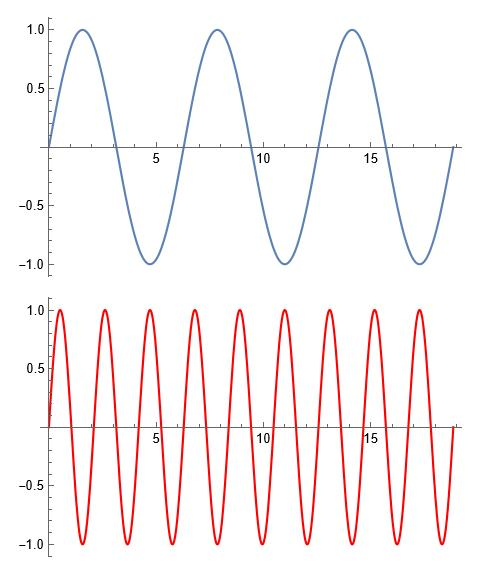
\includegraphics[scale=0.4]{Imagenes/Tono_01.jpg}
\end{figure}
\end{frame}
\begin{frame}
\frametitle{Actividad a realizar}
Visita el sitio:

\href{https://www.youtube.com/watch?v=qNf9nzvnd1k}{https://www.youtube.com/watch?v=qNf9nzvnd1k}

Registra en tu cuaderno el valor de la frecuencia en la cual comenzaste a escuchar la señal, así como el valor de frecuencia en el cual dejaste de escuchar.
\end{frame}

\subsection{Timbre}

\begin{frame}
\frametitle{¿Qué es el timbre?}
El \textocolor{darkelectricblue}{cualidad que posibilita identificar} la fuente sonora, aunque
distintos instrumentos produzcan sonidos con el mismo tono e intensidad.
\end{frame}
\begin{frame}
\frametitle{El timbre en sonido}
Lo anterior es posible, pues el tono fundamental siempre va acompañado de \textocolor{darkmagenta}{tonos armónicos} llamados sobretonos, éstos le dan el timbre característico a un instrumento musical o a la voz.
\end{frame}
\begin{frame}
\frametitle{El timbre en sonido}
Por eso, podemos identificar las voces de personas conocidas, así como los instrumentos que producen un sonido.
\end{frame}

\section{Ejercicio}
\frame{\tableofcontents[currentsection, hideothersubsections]}
\subsection{Ejercicio 1}

\begin{frame}
\frametitle{Intensidad de sonido en una calle}
En una esquina congestionada, el nivel de sonido es de \SI{75}{\dB}. ¿Cuál es la intensidad del sonido aquí?
\end{frame}
\begin{frame}
\frametitle{Solución al Ejercicio 1}
\textocolor{red}{Datos}:
\pause
\begin{align*}
B &= \SI{75}{\dB} \\[0.5em]
I_{0} &= \SI{1d-12}{\watt\per\square\meter} \\[0.5em]
I &= \, ?
\end{align*}
\end{frame}
\begin{frame}
\frametitle{Solución al Ejercicio 1}
\textocolor{red}{Expresión}:
\pause
\begin{eqnarray*}
\begin{aligned}
B &= 10 \, \log \dfrac{I}{I_{0}} \pause \hspace{1cm} \Rightarrow \hspace*{0.2cm} \log \left( \dfrac{I}{I_{0}} \right) &= \dfrac{B}{10} \\[0.4em] \pause
\dfrac{I}{I_{0}} &= 10^{B/10} \\[0.4em] \pause
\Rightarrow \hspace*{0.2cm} I &= I_{0} \, 10^{B/10}
\end{aligned}
\end{eqnarray*}
\end{frame}
\begin{frame}
\frametitle{Solución al Ejercicio 1}
\textocolor{red}{Sustitución:}
\pause
\begin{eqnarray*}
\begin{aligned}
I &= (\SI{1d-12}{\watt\per\square\meter})(10^{7.5}) = \\[0.5em] \pause
I &= \SI{3.1622d-5}{\watt\per\square\meter}
\end{aligned}
\end{eqnarray*}
\end{frame}

\subsection{Ejercicio 2}

\begin{frame}
\frametitle{Enunciado del Ejercicio 2}
Un trompetista toca con un nivel de sonido de \SI{75}{\dB}. 
\\
\bigskip
\pause Se agregan tres trompetistas con la misma intensidad.
\\
\bigskip
\pause
¿Cuál es el nuevo nivel de sonido?
\end{frame}
\begin{frame}
\frametitle{Resolviendo el Ejercicio 2}
\textocolor{red}{Datos}:
\pause
\begin{eqnarray*}
\begin{aligned}
B &= \SI{75}{\dB} \hspace{0.3cm} \text{1 trompetista} \\[0.5em] \pause
B^{\prime} &= \, ? \hspace{0.3cm} \text{4 trompetistas}
\end{aligned}
\end{eqnarray*}
\end{frame}
\begin{frame}
\frametitle{Resolviendo el Ejercicio 2}
\textocolor{red}{Expresión:}
\pause
\begin{align*}
B = 10 \,\log \left( \dfrac{I_{1}}{I_{0}} \right)
\end{align*}
\end{frame}
\begin{frame}
\frametitle{Resolviendo el Ejercicio 2}
La intensidad de cuatro trompetas es cuatro veces la intensidad de una trompeta, \pause es decir, $4 \, I_{1}$.
\end{frame}
\begin{frame}
\frametitle{Resolviendo el Ejercicio 2}
El nivel de sonido de las cuatro trompetas sería:
\pause
\begin{eqnarray*}
\begin{aligned}
B^{\prime} &= 10 \, \log \left( \dfrac{4 \, I_{1}}{I_{0}} \right) = \pause 10 \, \log \left( 4 \cdot \dfrac{I_{1}}{I_{0}} \right) = \\[0.5em] \pause
&= 10 \, \log \, 4 + 10 \, \log \left( \dfrac{I_{1}}{I_{0}} \right) = \\[0.5em] \pause
&= \SI{6.0}{\dB} + \SI{75}{\dB} = \pause \SI{85}{\dB}
\end{aligned}
\end{eqnarray*}
\end{frame}

\section{Intensidad sonido y distancia}
\frame{\tableofcontents[currentsection, hideothersubsections]}
\subsection{Relación entre variables}

\begin{frame}
\frametitle{Intensidad y distancia}
Normalmente la intensidad de un sonido \textocolor{red}{disminuye al alejarse} uno de la fuente del
sonido.
\end{frame}
\begin{frame}
\frametitle{Intensidad y distancia}
En habitaciones cerradas, el efecto se altera debido a la reflexión de las paredes.
\end{frame}
\begin{frame}
\frametitle{Intensidad y distancia}
No obstante, si una fuente está al aire libre, de manera que el sonido pueda radiarse libremente en todas direcciones, \pause la intensidad \textocolor{carmine}{decrece según el inverso del cuadrado de la distancia}:
\pause
\begin{align*}
B \propto \dfrac{1}{r^{2}}
\end{align*}
\end{frame}
\begin{frame}
\frametitle{Ejercicio a resolver}
El nivel de sonido de un avión a chorro a una distancia de \SI{30}{\meter} es de \SI{140}{\dB}
\\
\bigskip
\pause
¿Cuál será el nivel de sonido a \SI{300}{\meter}? (Desprecia las reflexiones del suelo).
\end{frame}
\begin{frame}
\frametitle{Planteamiento previo}
Dado el nivel del sonido, podemos determinar la intensidad a \SI{30}{\meter} con la ecuación:
\pause
\begin{align*}
B = 10 \,\log \left( \dfrac{I_{1}}{I_{0}} \right)
\end{align*}
\end{frame}
\begin{frame}
\frametitle{Planteamiento previo}
Puesto que la intensidad disminuye con el cuadrado de la distancia, ignorando las reflexiones, podemos encontrar $I$ a \SI{300}{\meter} \pause y de nuevo aplicar la ecuación anterior para obtener el nivel de sonido.
\end{frame}
\begin{frame}
\frametitle{Obteniendo la intensidad}
La intensidad $I$ a \SI{30}{\meter} es:
\pause
\begin{eqnarray*}
\begin{aligned}
\SI{140}{\dB} &= 10 \, \log \left( \dfrac{I}{\SI{1d-12}{\watt\per\square\meter}} \right) = \\[0.5em] \pause
\SI{14}{\dB} &= \log \left( \dfrac{I}{\SI{1d-12}{\watt\per\square\meter}} \right)
\end{aligned}
\end{eqnarray*}
\end{frame}
\begin{frame}
\frametitle{Aprovechando los logaritmos}
Elevamos ambos lados de la ecuación a la potencia $10$:
\pause
\begin{eqnarray*}
\begin{aligned}
10^{14} &= \dfrac{I}{\SI{1d-12}{\watt\per\square\meter}} \\[0.5em] \pause
I &= (10^{14})(\SI{1d-12}{\watt\per\square\meter}) = \\[0.5em] \pause
I &= \SI{d2}{\watt\per\square\meter}
\end{aligned}
\end{eqnarray*}
\end{frame}
\begin{frame}
\frametitle{Calculando la intensidad}
A \SI{300}{\meter}, que es una \textocolor{cobalt}{distancia diez veces más lejos}, \pause la intensidad será:
\pause
\begin{eqnarray*}
\begin{aligned}
\left( \dfrac{1}{10} \right)^{2} = \pause \dfrac{1}{100}
\end{aligned}
\end{eqnarray*}
\pause
por lo que:
\begin{align*}
I^{\prime} = \SI{1}{\watt\per\square\meter}
\end{align*}
\end{frame}
\begin{frame}
\frametitle{Valor de B a \SI{300}{m}}
El nivel de sonido es:
\pause
\begin{eqnarray*}
\begin{aligned}
B^{\prime} &= 10 \, \log \left( \dfrac{\SI{1}{\watt\per\square\meter}}{\SI{1d-12}{\watt\per\square\meter}} \right) = \\[0.5em] \pause
&= \SI{120}{\dB}
\end{aligned}
\end{eqnarray*}
\end{frame}
\begin{frame}
\frametitle{Conclusión}
A \SI{300}{\meter}, el sonido está en el umbral del dolor.
\\
\bigskip
\pause
Por ello, los trabajadores en aeropuertos cubren sus oídos para protegerlos de daños.
\end{frame}

\section{Efecto Doppler}
\frame[allowframebreaks]{\tableofcontents[currentsection, hideothersubsections]}
\subsection{Definición}

\begin{frame}
\frametitle{Propagación del sonido}
\vspace*{-1cm}
\begin{figure}
    \centering
    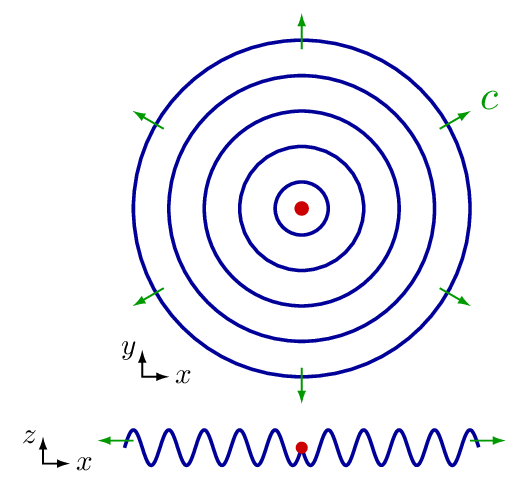
\includegraphics[scale=0.35]{Imagenes/Efecto_Doppler_01.png}
\end{figure}
\end{frame}
\begin{frame}
\frametitle{Propagación del sonido}
\vspace*{-1cm}
\begin{figure}
    \centering
    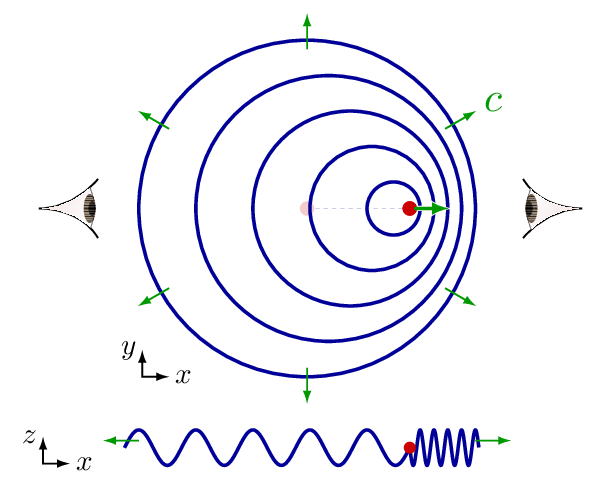
\includegraphics[scale=0.35]{Imagenes/Efecto_Doppler_02.png}
\end{figure}
\end{frame}
\begin{frame}
\frametitle{Entendiendo el fenómeno}
Este fenómeno se aprecia claramente al escuchar la sirena de una ambulancia, \pause pues notamos que el tono se hace \textocolor{byzantium}{agudo a medida que se aproxima} \pause y después se \textocolor{coquelicot}{hace grave al alejarse}.
\end{frame}
\begin{frame}
\frametitle{Entendiendo el fenómeno}
Cuando la fuente sonora se \textocolor{ao(english)}{acerca al observador}, las ondas que emite tienden a alcanzar a las que se desplazan delante de ellas, \pause \textocolor{ao(english)}{reduciendo la longitud de onda}.
\end{frame}
\begin{frame}
\frametitle{Entendiendo el fenómeno}
Lo cual provoca un aumento en la frecuencia del sonido; por esta razón se escucha un sonido agudo.
\end{frame}
\begin{frame}
\frametitle{Entendiendo el fenómeno}
\vspace*{-1cm}
\begin{figure}
    \centering
    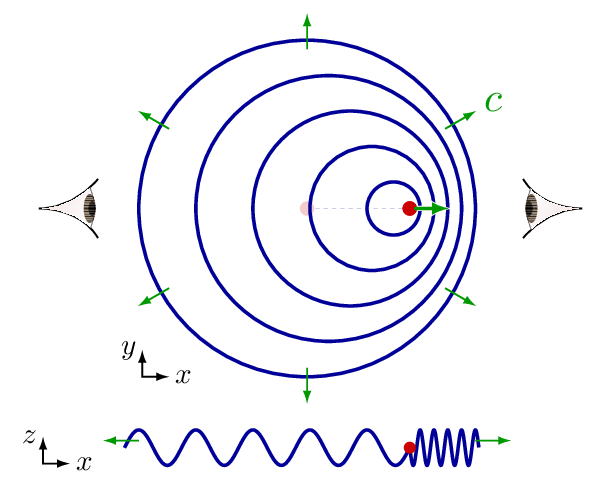
\includegraphics[scale=0.35]{Imagenes/Efecto_Doppler_02.png}
\end{figure}
\end{frame}
\begin{frame}
\frametitle{Entendiendo el fenómeno}
Al \textocolor{red}{alejarse}, la distancia entre crestas aumenta y origina una \textocolor{red}{disminución en la frecuencia}; \pause debido a ello se escucha un sonido grave.
\end{frame}
\begin{frame}
\frametitle{¿Y si la fuente está fija?}
Sucede un efecto similar si la fuente sonora \textocolor{cobalt}{permanece fija} y el observador es quien se acerca; \pause éste percibe una frecuencia mayor porque le llegan más ondas sonoras por unidad de tiempo, reduciéndose la longitud de onda.
\end{frame}
\begin{frame}
\frametitle{¿Y si la fuente está fija?}
Cuando el observador se aleja ocurre el efecto contrario.
\end{frame}
\begin{frame}
\frametitle{Definición del fenómeno}
El efecto Doppler consiste en un \textocolor{bulgarianrose}{cambio aparente en la frecuencia de un sonido}, durante el movimiento relativo entre el observador y la fuente sonora.
\end{frame}

\subsection{La frecuencia aparente}

\begin{frame}
\frametitle{Estimando la frecuencia}
Para calcular la frecuencia aparente de un sonido que escucha un observador, tenemos las siguientes situaciones:
\pause
\setbeamercolor{item projected}{bg=aquamarine,fg=black}
\setbeamertemplate{enumerate items}{%
\usebeamercolor[bg]{item projected}%
\raisebox{1.5pt}{\colorbox{bg}{\color{fg}\footnotesize\insertenumlabel}}%
}
\begin{enumerate}[<+->]
\item Fuente en movimiento y el observador fijo.
\item Fuente fija y el observador en movimiento.
\end{enumerate}
\end{frame}
\begin{frame}
\frametitle{Fuente en movimiento}
La expresión que nos determina la frecuencia aparente cuando la fuente sonora está en movimiento y el observador en reposo es:
\pause
\begin{align*}
\pderivada{f} = \dfrac{f \, V}{V \pm v}
\end{align*}
\end{frame}
\begin{frame}
\frametitle{Fuente en movimiento}
\vspace*{-1cm}
\begin{align*}
\pderivada{f} = \dfrac{f \, V}{V \pm v}
\end{align*}
donde:
\pause
\setbeamercolor{item projected}{bg=bananayellow,fg=ao}
\setbeamertemplate{enumerate items}{%
\usebeamercolor[bg]{item projected}%
\raisebox{1.5pt}{\colorbox{bg}{\color{fg}\footnotesize\insertenumlabel}}%
}
\begin{enumerate}[<+->]
\item $\pderivada{f}$ es la frecuencia aparente.
\item $f$ frecuencia real emitida por la fuente.
\item $V$ velocidad de propagación del sonido (\unit{\meter\per\second}).
\item $v$ velocidad a la que se mueve la fuente sonora.
\end{enumerate}
\end{frame}
\begin{frame}
\frametitle{Observando el signo}
El \textocolor{ao}{signo menos} de la expresión se utiliza si la fuente sonora \textocolor{ao}{se acerca al observador}, \pause y el \textocolor{auburn}{signo más cuando se aleja de él}.
\end{frame}
\begin{frame}
\frametitle{Fuente en reposo}
Si la fuente sonora permanece en reposo y el observador es quien se acerca o aleja de ella, se usa la expresión:
\pause
\begin{align*}
\pderivada{f} = \dfrac{f \, (V \pm v)}{V}
\end{align*}
\end{frame}
\begin{frame}
\frametitle{El signo en la expresión}
El \textocolor{blue-violet}{signo más} de la expresión se utiliza si \textocolor{blue-violet}{el observador se acerca a la fuente sonora}, \pause y el signo menos cuando se aleja de ella.
\end{frame}
\begin{frame}
\frametitle{Ejercicio}
Una ambulancia lleva una velocidad cuya magnitud es de \SI{70}{\kilo\meter\per\hour} y su sirena suena con una frecuencia de \SI{830}{\hertz}.
\end{frame}
\begin{frame}
\frametitle{Ejercicio}
Qué frecuencia aparente escucha un observador que está parado, cuando:
\setbeamercolor{item projected}{bg=aquamarine,fg=black}
\setbeamertemplate{enumerate items}{%
\usebeamercolor[bg]{item projected}%
\raisebox{1.5pt}{\colorbox{bg}{\color{fg}\footnotesize\insertenumlabel}}%
}
\begin{enumerate}[<+->]
\item La ambulancia se acerca a él.
\item La ambulancia se aleja de él.
\end{enumerate}
Considera la velocidad del sonido en el aire con una magnitud de \SI{340}{\meter\per\second}.
\end{frame}
\begin{frame}
\frametitle{Solución al Ejercicio}
\textocolor{red}{Datos:}
\pause
\begin{align*}
v &= \SI{70}{\kilo\meter\per\hour} \\
f &= \SI{830}{\hertz} \\
V &= \SI{340}{\meter\per\second} \\
f^{\prime} &= \, ?
\end{align*}
\end{frame}
\begin{frame}
\frametitle{Solución al Ejercicio}
\textocolor{red}{Expresión:}    
\begin{align*}
\pderivada{f} = \dfrac{f \, V}{V \pm v}
\end{align*}
\end{frame}
\begin{frame}
\frametitle{Revisando los casos}
Primer caso: la ambulancia \textocolor{darkgreen}{se acerca} al observador:
\pause
\begin{align*}
\pderivada{f} = \dfrac{f \, V}{V - v}
\end{align*}
\end{frame}
\begin{frame}
\frametitle{Revisando los casos}
Segundo caso: la ambulancia \textocolor{darkmagenta}{se aleja} al observador:
\pause
\begin{align*}
\pderivada{f} = \dfrac{f \, V}{V + v}
\end{align*}
\end{frame}
\begin{frame}
\frametitle{Solución al Ejercicio}
Antes de ocupar la expresión, recordemos que es necesario manejar siempre las magnitudes con las \textocolor{blue}{unidades fundamentales}, en este caso, la velocidad expresarla en \unit{\meter\per\second}
\end{frame}
\begin{frame}
\frametitle{Haciendo la conversión}
Presentamos los factores de conversión:
\pause
\begin{eqnarray*}
\begin{aligned}
\SI{1}{\kilo\meter} &= \SI{1000}{\meter} \\[0.5em] \pause
\SI{1}{\hour} &= \SI{36000}{\second}
\end{aligned}
\end{eqnarray*}
\end{frame}
\begin{frame}
\frametitle{Haciendo la Conversión}
\begin{eqnarray*}
\begin{aligned}
v &= \SI[per-mode=fraction]{70}{\kilo\meter\per\hour} \left( \dfrac{\SI{1000}{\meter}}{\SI{1}{\kilo\meter}} \right) \left( \dfrac{\SI{1}{\hour}}{\SI{3600}{\second}} \right) = \\[0.5em] \pause
v &= \SI[per-mode=fraction]{19.44}{\meter\per\second}
\end{aligned}
\end{eqnarray*}
\end{frame}
\begin{frame}
\frametitle{Primer caso}
La ambulancia se acerca al observador:

\textocolor{red}{Sustitución:}
\pause
\begin{eqnarray*}
\begin{aligned}
\pderivada{f} &= \dfrac{(\SI{830}{\hertz})(\SI{340}{\meter\per\second})}{(\SI{340}{\meter\per\second}) - (\SI{19.44}{\meter\per\second})} = \\[0.5em] \pause
\pderivada{f} &= \dfrac{\SI[per-mode=fraction]{2.822d5}{\meter\per\square\second}}{\SI[per-mode=fraction]{320.56}{\meter\per\second}} = \pause \num{880.33} \dfrac{\unit{\meter\second}}{\unit{\meter\square\second}} = \pause \SI{880.33}{\hertz}
\end{aligned}
\end{eqnarray*}
\end{frame}
\begin{frame}
\frametitle{Segundo caso}
La ambulancia se aleja al observador:

\textocolor{red}{Sustitución:}
\pause
\begin{eqnarray*}
\begin{aligned}
\pderivada{f} &= \dfrac{(\SI{830}{\hertz})(\SI{340}{\meter\per\second})}{(\SI{340}{\meter\per\second}) + (\SI{19.44}{\meter\per\second})} = \\[0.5em] \pause
\pderivada{f} &= \dfrac{\SI[per-mode=fraction]{2.822d5}{\meter\per\square\second}}{\SI[per-mode=fraction]{359.44}{\meter\per\second}} = \pause \num{785.11} \dfrac{\unit{\meter\second}}{\unit{\meter\square\second}} = \pause \SI{785.11}{\hertz}
\end{aligned}
\end{eqnarray*}
\end{frame}
\begin{frame}
\frametitle{Enunciado segundo ejercicio}
Un automovilista que viaja a una velocidad cuya magnitud es de \SI{80}{\kilo\meter\per\hour} escucha el silbato de una fábrica cuya frecuencia es de \SI{1100}{\hertz}.
\end{frame}
\begin{frame}
\frametitle{Enunciado segundo ejercicio}
Calcular la frecuencia aparente escuchada por el automovilista cuando:
\pause
\setbeamercolor{item projected}{bg=bronze,fg=black}
\setbeamertemplate{enumerate items}{%
\usebeamercolor[bg]{item projected}%
\raisebox{1.5pt}{\colorbox{bg}{\color{fg}\footnotesize\insertenumlabel}}%
}
\begin{enumerate}[<+->]
\item Se acerca a la fuente.
\item Se aleja de la fuente.
\end{enumerate}
\pause
Considera la magnitud de la velocidad de propagación del sonido en el aire es de \SI{340}{\meter\per\second}.
\end{frame}
\begin{frame}
\frametitle{Solución al Ejercicio}
\textocolor{red}{Datos:}
\pause
\begin{align*}
v &= \SI{80}{\kilo\meter\per\hour} = \SI{22.22}{\meter\per\second} \\
f &= \SI{1100}{\hertz} \\
V &= \SI{340}{\meter\per\second} \\
f^{\prime} &= \, ?
\end{align*}
\end{frame}
\begin{frame}
\frametitle{Solución al Ejercicio}
\textocolor{red}{Expresión:}    
\begin{align*}
\pderivada{f} = \dfrac{f \, (V \pm v)}{V}
\end{align*}
\end{frame}
\begin{frame}
\frametitle{Revisando los casos}
Primer caso: el observador \textocolor{darkslateblue}{se acerca} a la fuente sonora:
\pause
\begin{align*}
\pderivada{f} = \dfrac{f \, (V + v)}{V}
\end{align*}
\end{frame}
\begin{frame}
\frametitle{Revisando los casos}
Segundo caso: el observador \textocolor{bole}{se aleja} de la fuente sonora:
\pause
\begin{align*}
\pderivada{f} = \dfrac{f \, (V - v)}{V}
\end{align*}
\end{frame}
\begin{frame}
\frametitle{Primer caso}
El automovilista se acerca a la fuente sonora:

\textocolor{red}{Sustitución:}
\pause
\begin{eqnarray*}
\begin{aligned}
\pderivada{f} &= \dfrac{(\SI{1100}{\hertz})(\SI{340}{\meter\per\second} + \SI{22.22}{\meter\per\second})}{\SI{340}{\meter\per\second}} = \\[0.5em] \pause
\pderivada{f} &= \dfrac{\SI[per-mode=fraction]{398442}{\meter\per\square\second}}{\SI[per-mode=fraction]{340}{\meter\per\second}} = \pause \num{1171.88} \dfrac{\unit{\meter\second}}{\unit{\meter\square\second}} = \pause \SI{1171.88}{\hertz}
\end{aligned}
\end{eqnarray*}
\end{frame}
\begin{frame}
\frametitle{Segundo caso}
El automovilista se aleja a la fuente sonora:

\textocolor{red}{Sustitución:}
\pause
\begin{eqnarray*}
\begin{aligned}
\pderivada{f} &= \dfrac{(\SI{1100}{\hertz})(\SI{340}{\meter\per\second} - \SI{22.22}{\meter\per\second})}{\SI{340}{\meter\per\second}} = \\[0.5em] \pause
\pderivada{f} &= \dfrac{\SI[per-mode=fraction]{352735.8}{\meter\per\square\second}}{\SI[per-mode=fraction]{340}{\meter\per\second}} = \pause \SI{1037.45}{\hertz}
\end{aligned}
\end{eqnarray*}
\end{frame}
    
\end{document}

